% GURPS is a trademark of Steve Jackson Games, and its rules and art are
% copyrighted by Steve Jackson Games. All rights are reserved by Steve Jackson
% Games. This game aid is the original creation of Nathanael Farley and is
% released for free distribution, and not for resale, under the permissions
% granted in the Steve Jackson Games Online Policy.

\documentclass{article}
\usepackage[british]{babel}
\usepackage[margin=1in]{geometry}
\usepackage{graphicx}
\usepackage{nopageno}
\usepackage[sfdefault,condensed]{universalis}
\usepackage{caption}
\usepackage{fancyhdr}
\usepackage{hyperref}

\usepackage{gurps} % Download from https://github.com/nasfarley88/gurps-latex-package 
\usepackage{gurps-weaponcard}


\pagestyle{fancy}
\chead{Weapons cards for \gurps -- See more at \url{https://3d6andgo.blogspot.com/}}
\cfoot{\footnotesize\SJGamesOnlinePolicyGameAid{Nathana\null el Farley}}

\title{Weapon cards for \gurps}
\author{Nathana\null el Farley}
\begin{document}%

\maketitle

\noindent
This is a demonstration of the \texttt{gurps-weaponcard} package. More info can
be found at \url{https://3d6andgo.blogspot.com/2018/04/weapons-cards.html}. For
the code, see \url{https://github.com/nasfarley88/3d6andgo-stuff/tree/master/weaponsheet}.

\section*{Disclaimer}
\label{sec:disclaimer}

\SJGamesOnlinePolicyGameAid{Nathana\null el Farley}

\vfill

\begin{minipage}{\linewidth}
  \begin{center}
    \RangedWeaponCard{
      name={Cordite Pistol},
      acc=2,
      damage={3d pi},
      rof=1,
      range={100/1,000},
      bulk=2,
      shots=10+1(3),
      rcl=3,
      st=9,
      notes=,
      points=9,
      lc=2,
      weaponpic={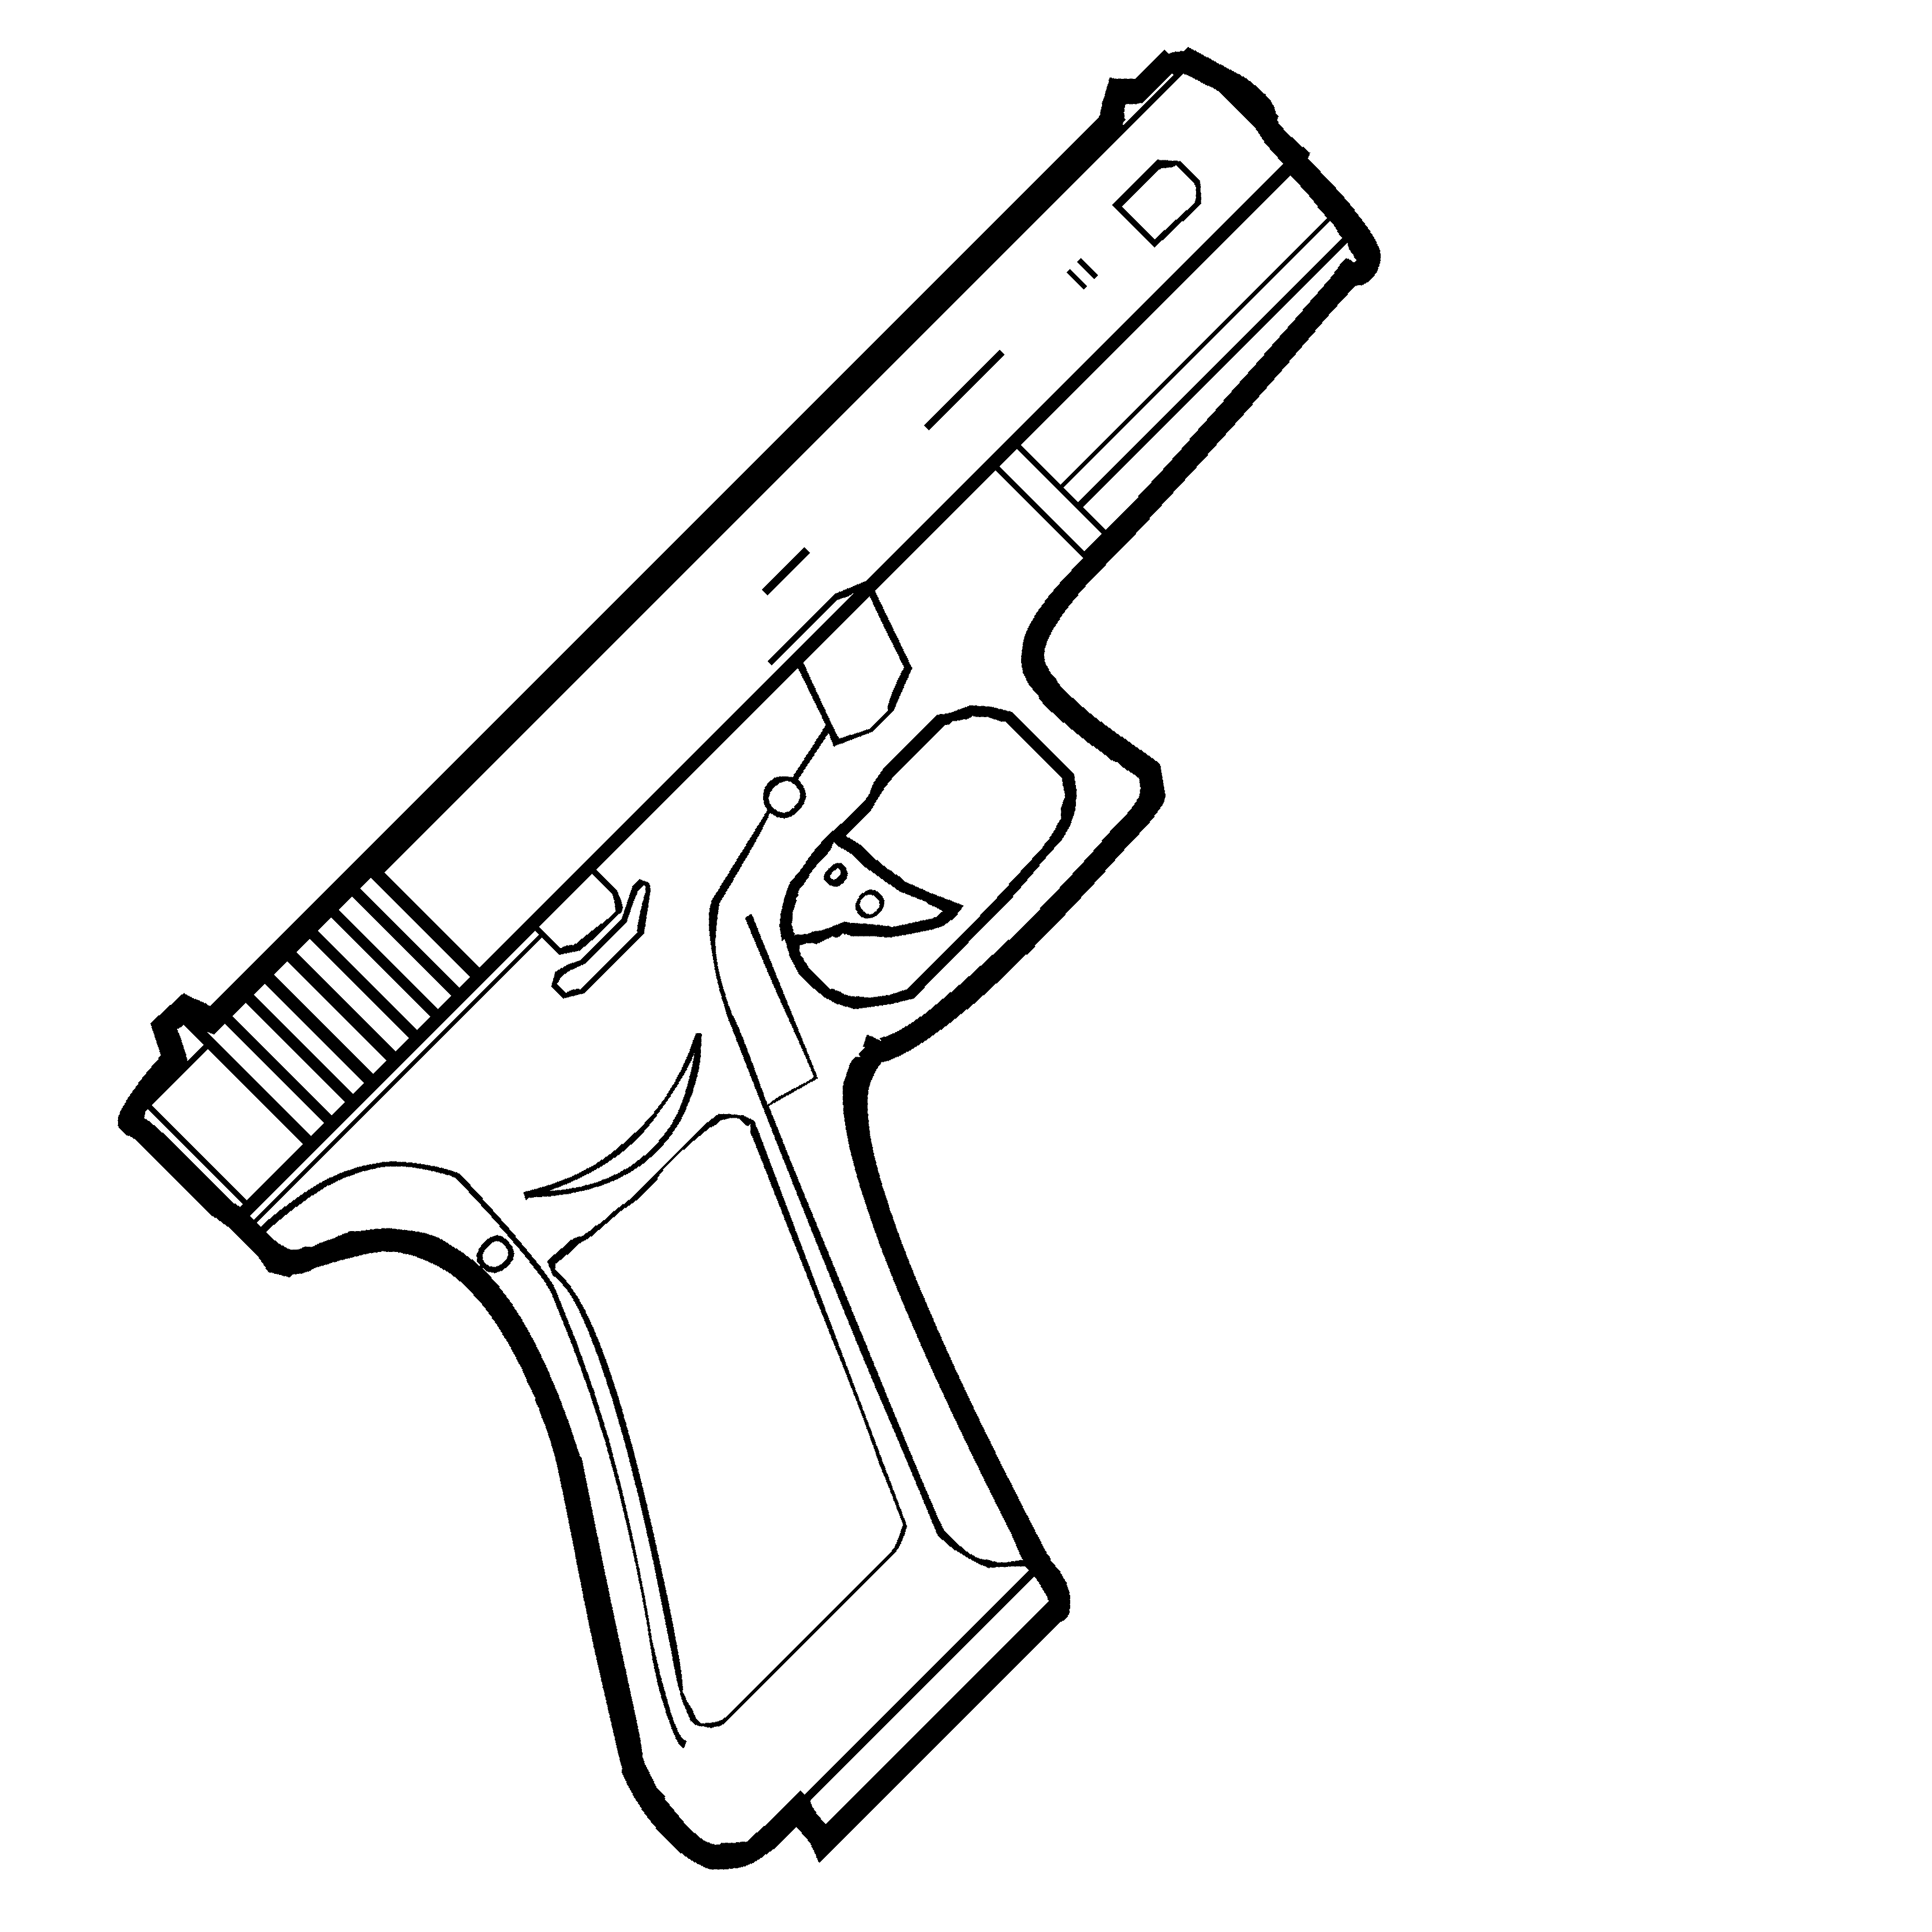
\includegraphics[width=2cm]{images/glock.pdf}}
    }%
    \RangedWeaponCard{
      name={Silenced Cordite Pistol},
      acc=2,
      damage={3d pi},
      rof=1,
      range={100/1,000},
      bulk=2,
      shots=10+1(3),
      rcl=3,
      st=9,
      notes=,
      points=10,
      lc=3,
      weaponpic={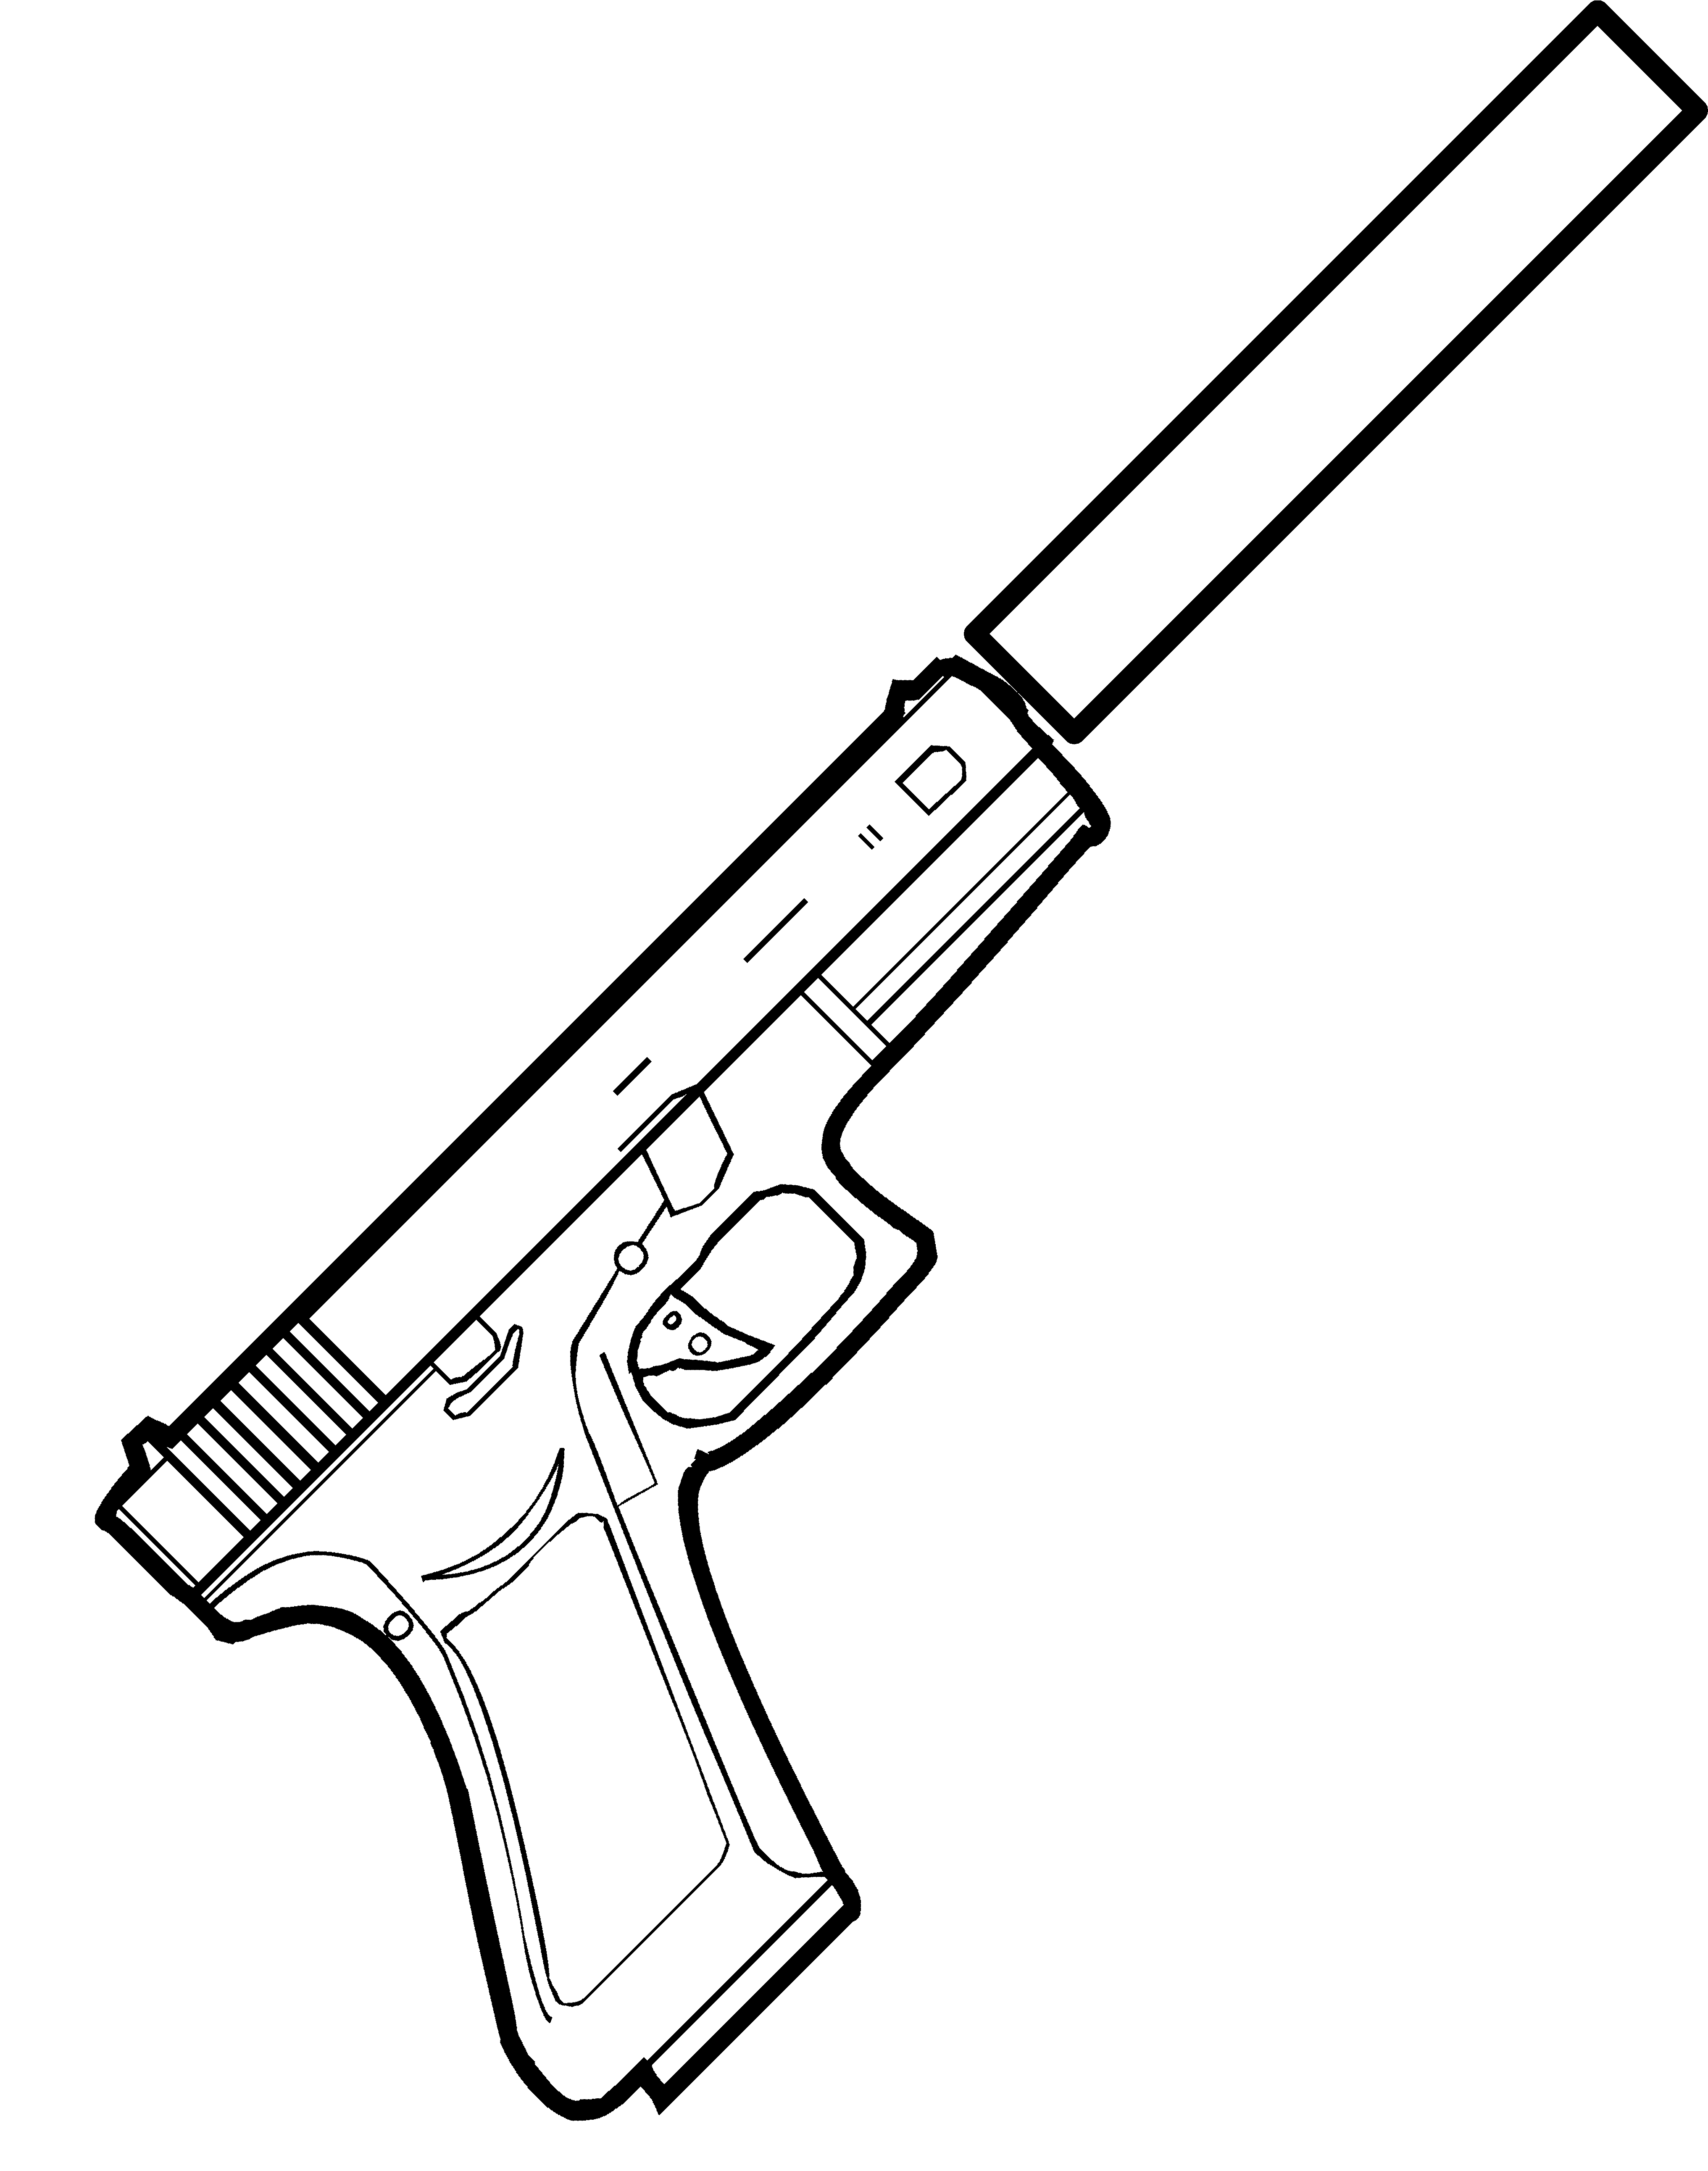
\includegraphics[width=1.5cm]{images/glocksilenced.pdf}}
    }

    \RangedWeaponCard{
      name={Cordite Rifle},
      acc=3,
      damage={6d pi},
      rof=1,
      range={100/1,000},
      bulk=2,
      shots=\scalebox{0.9}[1.0]{30+1(3)},
      rcl=2,
      st=9,
      notes=,
      points=26,
      lc=2,
      weaponpic={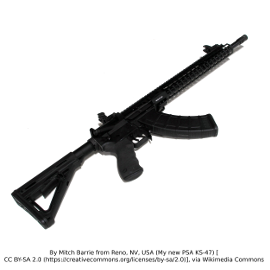
\includegraphics[width=1.9cm]{images/rifle.png}}
    }%
    \RangedWeaponCard{
      name={Silenced Cordite Rifle},
      acc=3,
      damage={6d pi},
      rof=1,
      range={100/1,000},
      bulk=2,
      shots=\scalebox{0.9}[1.0]{30+1(3)},
      rcl=2,
      st=9,
      notes=,
      points=27,
      lc=3,
      weaponpic={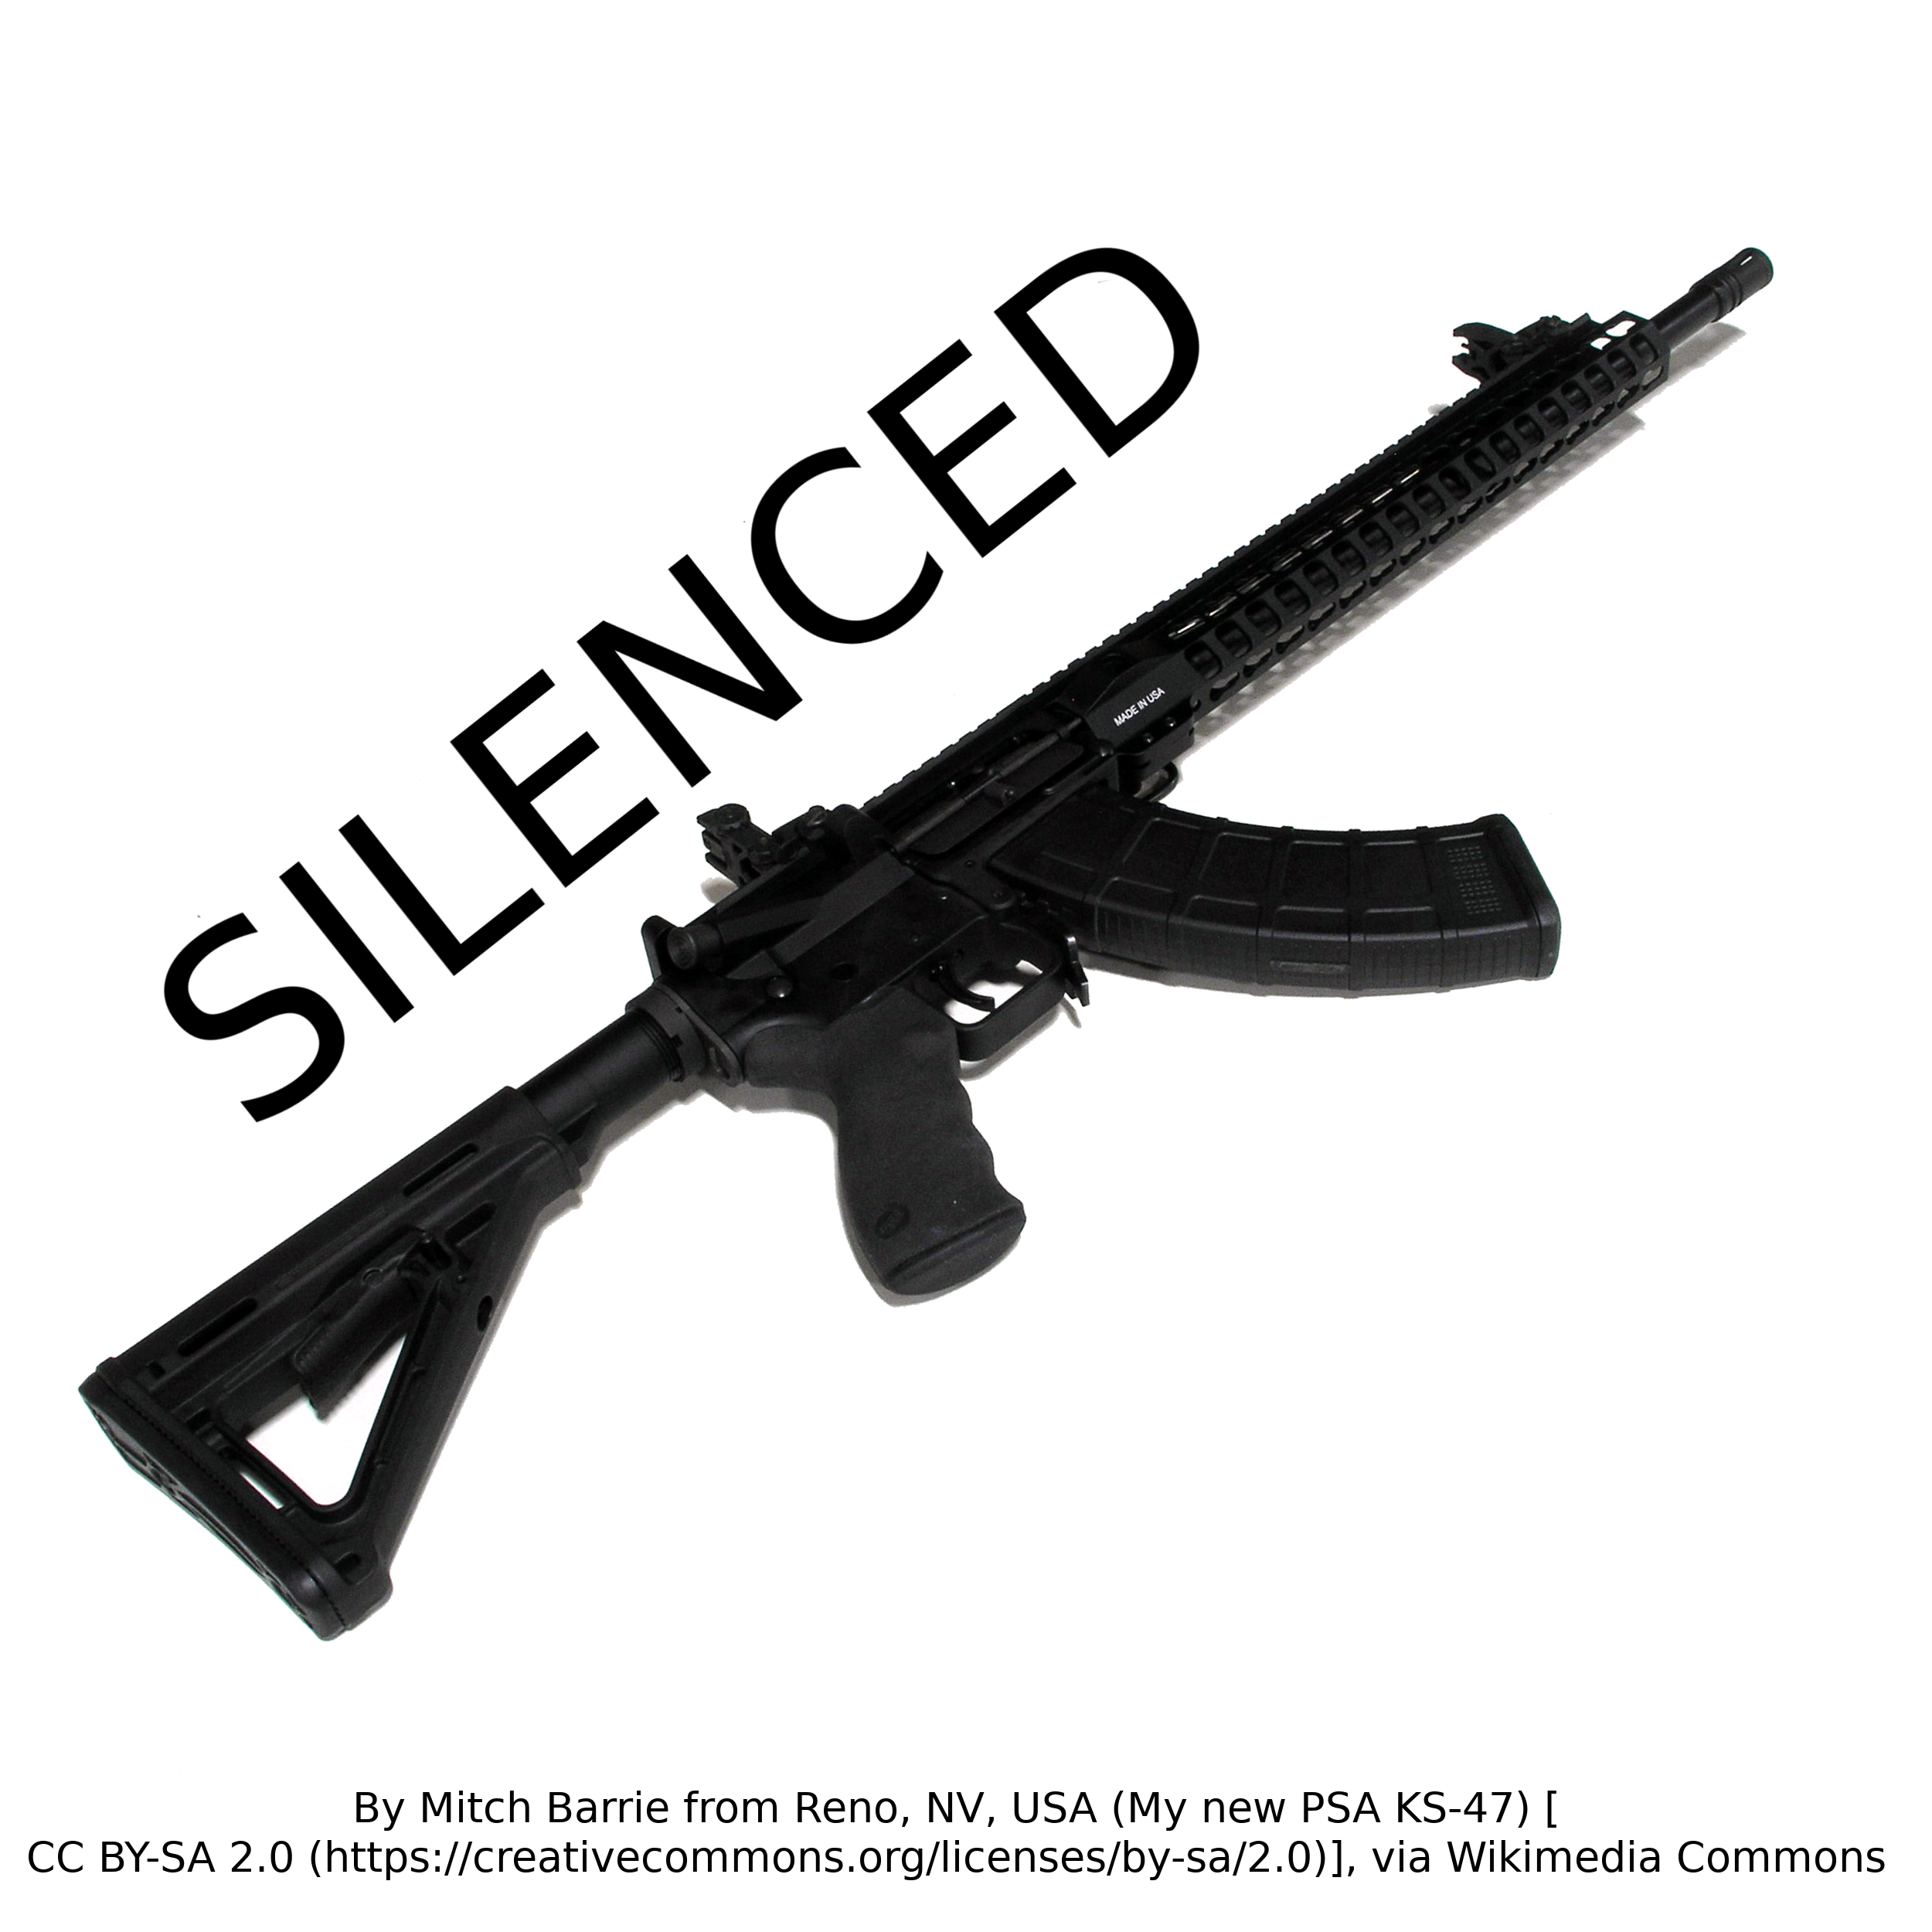
\includegraphics[width=1.9cm]{images/riflesilenced.png}}
    }

    \MeleeWeaponCard{
      name=katana-but-not,
      parry=0,
      damage=1d+2/1d+4,
      reach={\scalebox{0.9}[1.0]{1,2(cut only)}},
      st=8,
      lc=1,
      points=11,
      notes=,
      weaponpic={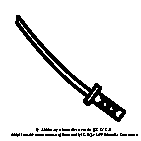
\includegraphics[width=1.9cm]{images/katanasword.pdf}}
    }% 
    \RangedWeaponCard{
      name={Sling},
      acc=0,
      damage={sw pi},
      rof=1,
      range={6x/10x},
      bulk=-4,
      shots=1(2),
      st=6,
      notes=,
      points=0\raisebox{1ex}{\small *},
      lc=0,
    }%
  \end{center}
  \captionof{figure}{A demonstration of the various possibilities. See the
    \texttt{weapons.tex} file, l.39, for code examples!}
\end{minipage}
\vfill
\NewDocumentCommand{\ul}{m}{\rule[-2pt]{#1}{0.3pt}}%
\clearpage\noindent\centering
\vspace*{\fill}%

\foreach \i in {1,...,8} {%
  \foreach \j in {1,2} {%
    \RangedWeaponCard{
      name=\ul{9.5em},
      damage=\ul{2em},
      acc=\ul{1em},
      rof=\ul{1em},
      range=\ul{4em},
      bulk=\ul{1em},
      shots=\ul{2em},
      rcl=\ul{1ex},
      st=\ul{2ex},
      lc=\ul{1ex},
      points=\rule{0pt}{1ex},
      cost=\ul{2em},
      weight=\ul{2em},
      notes=\ul{9.5em}
    }%
  }\\[-1pt]%
}%
\vfill%
\newpage%
\vspace*{\fill}%
\foreach \i in {1,...,8} {%
  \foreach \j in {1,2} {%
    \MeleeWeaponCard{
      name=\ul{9.5em},
      parry=\ul{1em},
      damage=\ul{2em},
      reach=\ul{2em},
      st=\ul{2ex},
      lc=\ul{1ex},
      points=\rule{0pt}{1ex},
      cost=\ul{2em},
      weight=\ul{2em},
      notes=\ul{9.5em}
    }%
  }\\[-1pt]%
}%
\vfill
\end{document}

%%% Local Variables:
%%% mode: latex
%%% TeX-master: "main"
%%% End:
